\documentclass{article}
\usepackage[utf8]{inputenc}

\title{TT3010 - Audiotechnology and Room Acoustics \\ Lab 2 - Loudspeaker measurements}
\author{Peter Svensson}
\date{\today}

\usepackage{natbib}
\usepackage{graphicx}
\usepackage{float}

\begin{document}

\maketitle

\begin{figure}[H]
\centering
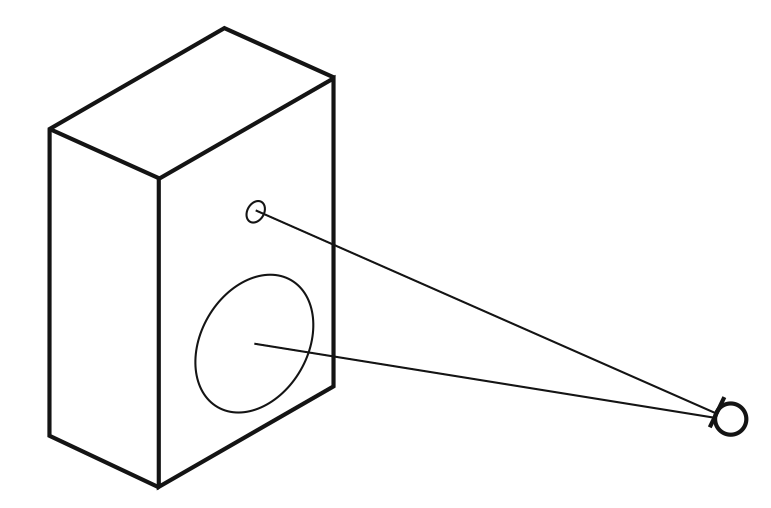
\includegraphics[scale=1]{figs/Twowaylsp.png}
\end{figure}

\section{Introduction}
\textbf{The goal is that you should understand how a loudspeaker's impulse response is related to its frequency response, and how the impulse response,
and other quantities can be measured.}

\section{Needed equipment in the anechoic room}

\begin{itemize}
    \item PC with measurement software and appropriate soundcard. This is usually always located outside the anechoic room.
     \item Measurement microphone, with a microphone stand, to be used inside the anechoic room.
     \item Loudspeaker to be tested, with a stand. This loudspeaker could either be a student's own loudspeaker, or one from the acoustics lab.
     \item Amplifier for the loudspeaker, unless it is built into the loudspeaker. 
     \item Measurement tape for measuring distance.
\end{itemize}

\section{Details}
The task is to use an impulse response measurement system (Easera, or WinMLS,
or similar) with  a measurement microphone to measure impulse response for a loudspeaker to be tested. 
Once an impulse response has been measured, the corresponding frequency response can be viewed. The software carries out an FFT on the impulse response, which gives the frequency response.

\section{Procedure}

In the anechoic room, the signal-to-noise ratio is usually more than adequate, compared to other measurement situations (in more ordinary rooms). 
 Still, it is good practice to use this procedure to adjust the gain settings:

\begin{itemize}
    \item [1.] Choose the settings for the measurement software (sampling frequency, input and output channels, sweep length, stimulus signal amplitude (output amplitude).
    \item[2.] Turn on the stimulus signal, and adjust the sound card gain + loudspeaker amplifier to give a loud but not too loud level from the loudspeaker. After this, don’t change the output gains!
    \item[3.] Put the microphone at the shortest distance that you will use. Adjust the microphone amplifier (or sound card gain) to as high as possible gain without overload. After this, don’t change the input gains!
\end{itemize}

\section{Theory}

\subsection{Relationship between the impulse response and the frequency response}

%\begin{figure}[H]
%    \centering
%    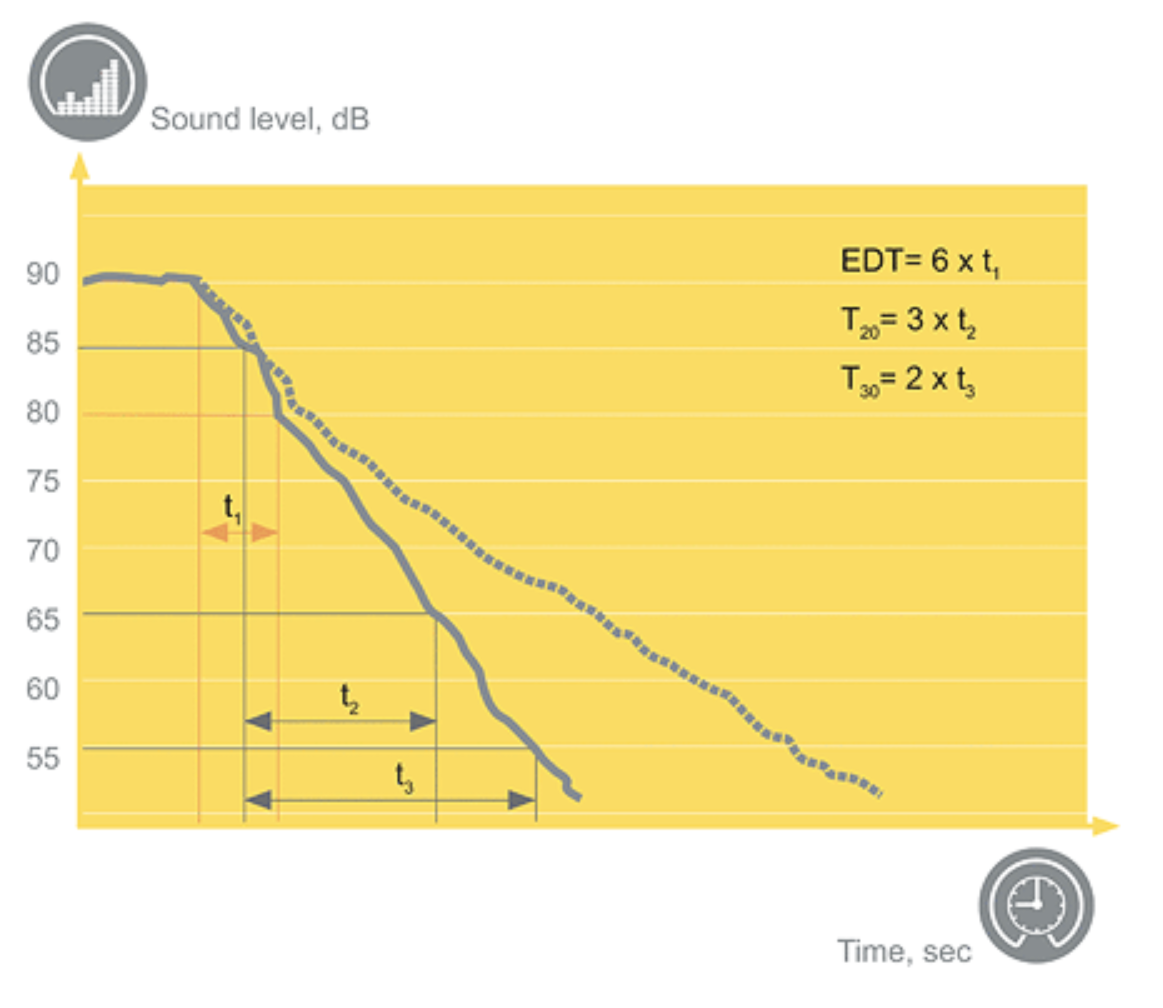
\includegraphics{edt_t20_t30.png}
%    \caption{Illustration showing how to calculate EDT, $T_{20}$ and $T_{30}$. From \cite{reverb}. This is done automatically by the measurement software, for one octave (or third-octave) band after another.}
%    \label{fig:reverb}
%\end{figure}


\section{Tasks}
\begin{itemize}
    \item [1.] Measure the impulse response at a distance of 1m in front of the loudspeaker, the so-called "on-axis" response, inside the anechoic room. \\
	View/plot the frequency response when the impulse response is cut:\\
    \begin{itemize}
	\item 1 ms after the direct sound
	\item 3 ms after the direct sound	
	\item 10 ms after the direct sound	
	\item 50 ms after the direct sound	
	\end{itemize}    
    \item [2.] Measure the impulse response at a distance of 1m from the center points of the woofer, in angles of 30, 60, 90 and 180 degrees relative to on-axis, inside the anechoic room. \\
    View/plot the frequency responses on top of each other. Can see you see the expected increase in directivity as the frequency increases? 
    \item [3.] Again, measure the on-axis response, 1m in front of the loudspeaker, inside the anechoic room, but now with a wooden board on the grid floor, to simulate a floor. \\
    View/plot two versions of the frequency response by cutting the impulse response:\\
    \begin{itemize}
	\item Immediately before the floor reflection
	\item Immediately after the floor reflection	
	\end{itemize}    
	What differences can you observe?
\end{itemize}

Write a  report on this, one per group, using the standardized lab report format.


\end{document}
